\section{Tecnologie}

\subsection{Introduzione}

\begin{frame}{Tecnologie utilizzate}

\begin{itemize}
\item JBoss AS (Application Server) 7.1
	\begin{itemize}
	
	\vspace{0.5em}
	
	\item fornisce l'infrastruttura per consentire \\
			l'esecuzione di una web application
	\end{itemize}

\vspace{1em}

\item Java EE (Java Platform, Enterprise Edition) 6
	\begin{itemize}
	
	\vspace{0.5em}
	
	\item piattaforma software per lo sviluppo di applicazioni enterprise
	
	\vspace{0.7em}
	
	\item comprende varie tecnologie, fra cui:
		\begin{itemize}
		
		\vspace{0.4em}
		
		\item JPA (Java Persistence API) 2.0
		
		\vspace{0.6em}
		
		\item CDI (Contexts and Dependency Injection) 1.0
		
		\vspace{0.6em}
		
		\item JSF (JavaServer Faces) 2.0
		\end{itemize}
		
	\end{itemize}

\end{itemize}


\end{frame}

\begin{frame}{Bean}

\begin{itemize}
\item Componenti software riusabili \\
	che possono essere gestiti dal container

\vspace{1em}

\item Principali specifiche:
	\begin{itemize}
	
	\vspace{0.8em}
	
	\item \textsl{Enterprise JavaBeans} (EJB) \\
		logica di business o persistenza
		
		\begin{itemize}
		
		\vspace{0.5em}
		
		\item session bean
		
		\vspace{0.3em}
		
		\item message-driven bean
		
		\vspace{0.3em}
		
		\item entity bean
		\end{itemize}
	
	\vspace{0.8em}
	
	\item  \textsl{Managed beans}\\
		livello di presentazione
	\end{itemize}

\end{itemize}

\end{frame}





\begin{frame}[fragile]{Iniezione di dipendenza-1}


\begin{lstlisting}[basicstyle={\tiny\ttfamily}]
public class MovieLister{
    private MovieFinder finder;
    
    public MovieLister() {
        finder = new MovieFinderImpl();
    }
    
    ...
}
\end{lstlisting}


\begin{figure}
	\centering
	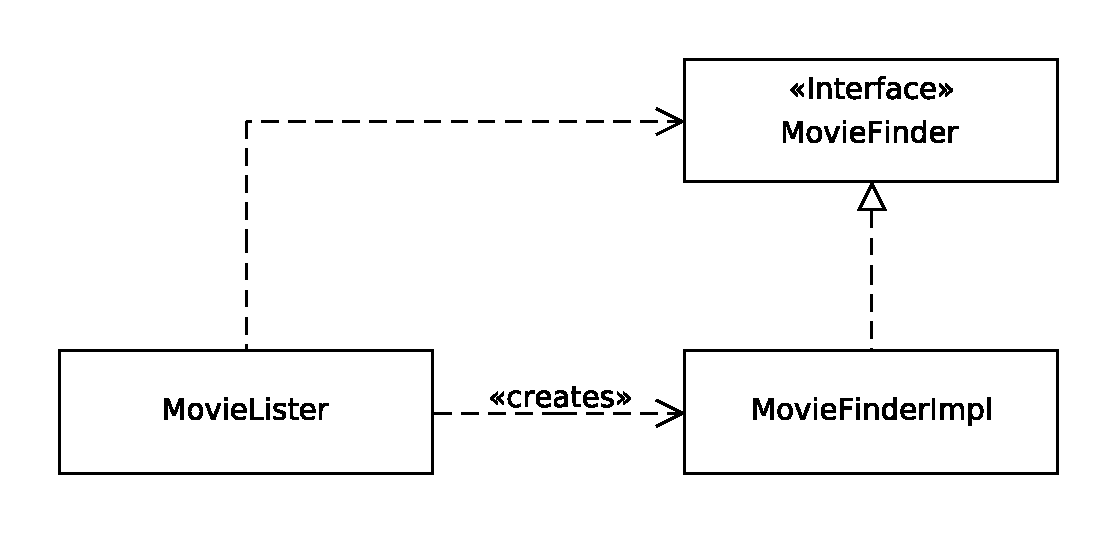
\includegraphics[width=0.5\textwidth]{fowler_no_DI.eps}
\end{figure}



\end{frame}



\begin{frame}[fragile]{Iniezione di dipendenza-2}


\begin{lstlisting}[basicstyle={\tiny\ttfamily}]
public class MovieLister{
    &&@Inject&& private MovieFinder finder;
    
    public MovieLister() {
    }
    
    ...
}
\end{lstlisting}


\begin{figure}
	\centering
	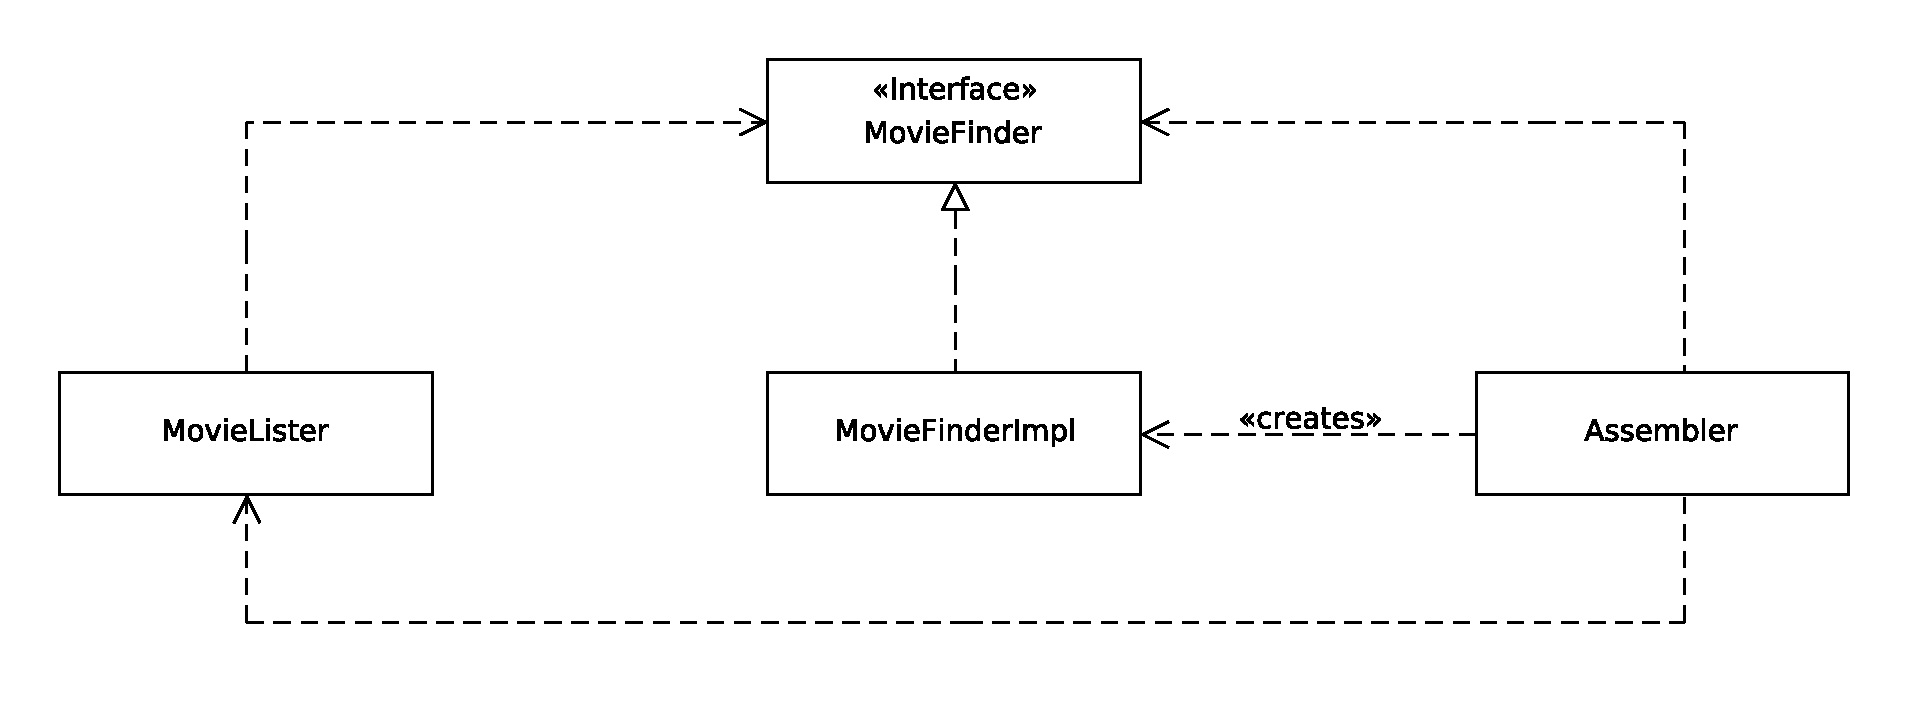
\includegraphics[width=0.7\textwidth]{fowler_DI.eps}
\end{figure}


\end{frame}




\subsection{JPA}
\begin{frame}{Java Persistence API}

\begin{itemize}
\item Applicazione \textsl{3-tier}:
\end{itemize}

\begin{figure}
	\centering
	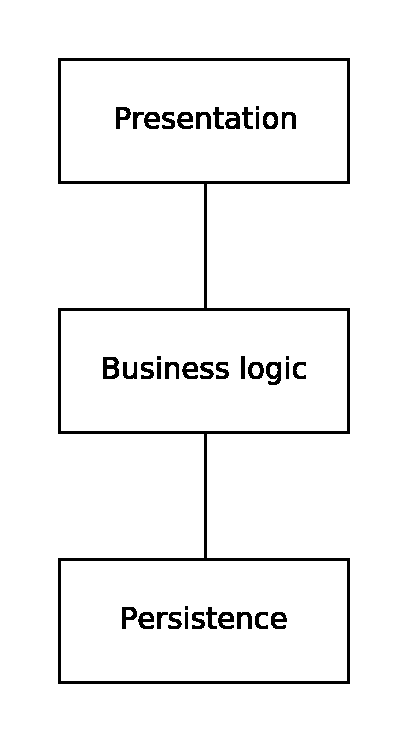
\includegraphics[width=0.2\textwidth]{3tier.eps}
\end{figure}

\end{frame}


\begin{frame}{\textsl{Object-relational impedance mismatch}}


\begin{itemize}

\vspace{0.4em}

\item Applicazione Java: \textsl{modello a oggetti}

\vspace{0.7em}

\item Database: \textsl{modello relazionale}

\end{itemize}

\begin{figure}
	\centering
	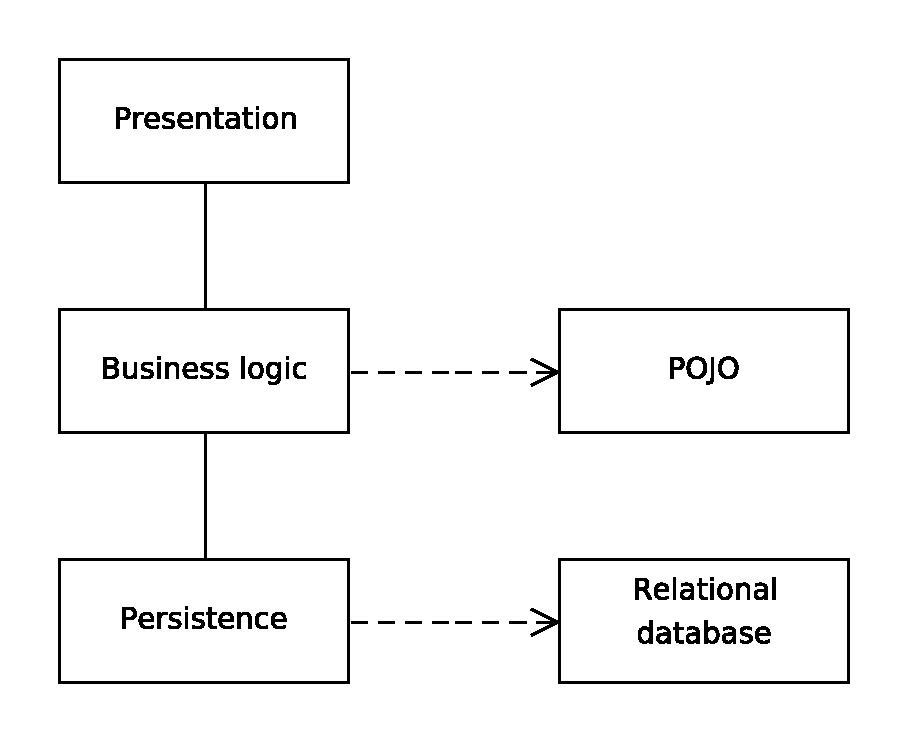
\includegraphics[width=0.5\textwidth]{3tier_entity.eps}
\end{figure}

\end{frame}




\begin{frame}{\textsl{Object-relational mapping}}

\begin{figure}
	\centering
	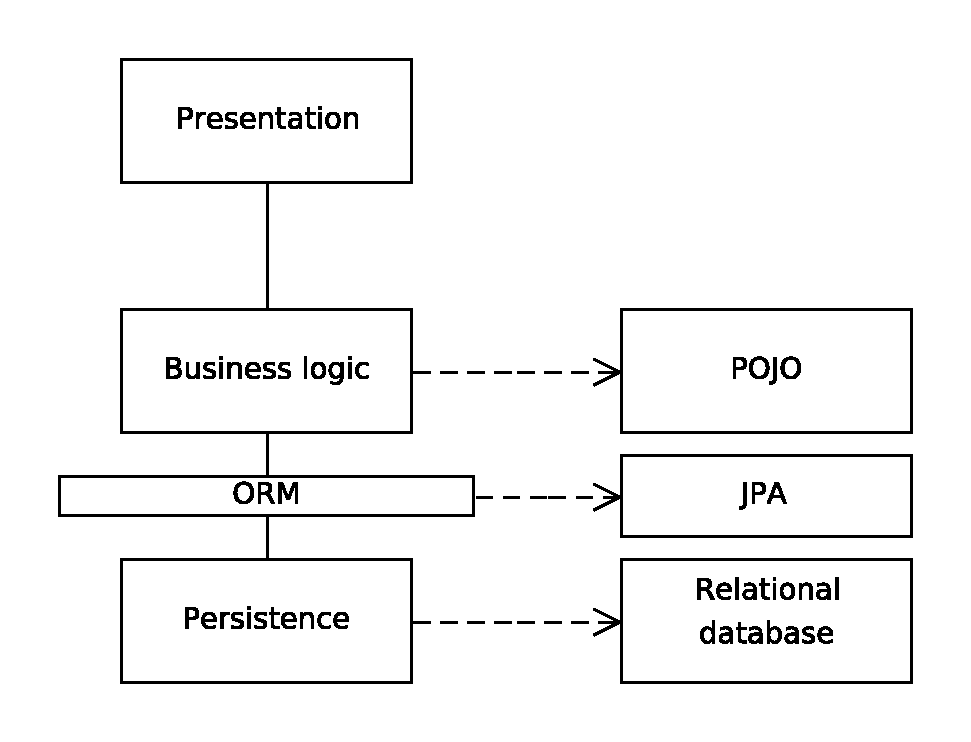
\includegraphics[width=0.5\textwidth]{3tier_orm.eps}
\end{figure}

\end{frame}



\begin{frame}[fragile]{Entità}


\begin{itemize}
\item Unità che possiede uno stato e può essere persistita

\vspace{0.6em}

\item una classe Java è un'entità se:
	\begin{itemize}
	
	\vspace{0.3em}
	
	\item è annotata \texttt{@Entity}
	
	\vspace{0.5em}
	
	\item ha un costruttore senza parametri non privato
	
	\vspace{0.5em}
	
	\item non è \texttt{final} e non possiede metodi o attributi \texttt{final}
	
	\vspace{0.5em}
	
	\item non possiede attributi pubblici
	\end{itemize}
\end{itemize}


\begin{lstlisting}[xleftmargin=0.3\textwidth,  basicstyle={\tiny\ttfamily}]
&&@Entity&&
public class Persona {
    private String nome, cognome;
    
    public Persona() {
        ...
    }
    ...
}
\end{lstlisting}



\end{frame}



\begin{frame}{Entity Manager}


\begin{itemize}
\item Gestisce le entità

\vspace{0.6em}

\item è associato ad un \textsl{Persistence Context}
	\begin{itemize}
	
	\vspace{0.3em}
	
	\item è l'insieme delle entità gestite da un Entity Manager \\
		in un dato momento
	
	\vspace{0.5em}
		
	\item se un entità fa parte di un Persistence Context viene detta \textsl{managed}
	
	\vspace{0.5em}
	
	\item altrimenti viene detta \textsl{detached}
	\end{itemize}
\end{itemize}

\begin{figure}
	\centering
	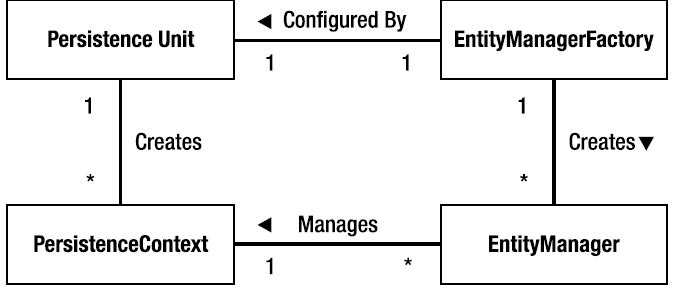
\includegraphics[width=0.5\textwidth]{JPA_concepts.png}
\end{figure}


\end{frame}

\begin{frame}{Query}

\begin{itemize}
\item Si usa il \textsl{Java Persistence Query Language} (JPQL)

\vspace{1em}

\item Sintassi simile a SQL, ma:

	\begin{itemize}
	
	\vspace{0.5em}
	
	\item è indipendente dal database
	
	\vspace{0.8em}
	
	\item utilizza le entità del modello di dominio e relativi attributi
	\end{itemize}

\vspace{1em}

\item Esempio:
	\begin{itemize}
	
	\vspace{0.5em}
	
	\item \texttt{SELECT p FROM Persona p}
	\end{itemize}

\end{itemize}

\end{frame}


\subsection{CDI}

\begin{frame}{Contexts and Dependency Injection}

\begin{itemize}
\item Problema: incompatibilità tra
	\begin{itemize}
	
	\vspace{0.5em}
	
	\item il livello di business, che usa EJB;
	
	\vspace{0.8em}
	
	\item il livello di presentazione, che usa Managed bean.
	\end{itemize}
	
\vspace{1em}	

\item CDI:
	\begin{itemize}
	
	\vspace{0.5em}
	
	\item consente l'utilizzo di EJB nel livello di presentazione
	
	\vspace{0.8em}
	
	\item include una specifica per la definizione di Managed bean
		\begin{itemize}
		
		\vspace{0.5em}
		
		\item integrazione con Expression Language (EL)
		\end{itemize}
	\end{itemize}
\end{itemize}

\end{frame}



\begin{frame}[fragile]{Contesto}

\begin{itemize}
\item Lo \textsl{scope} di un bean determina:

	\begin{itemize}
	
	\vspace{0.3em}
	
	\item il tempo di vita (\textsl{lifetime})
	
	\vspace{0.5em}
	
	\item la visibilità
	\end{itemize}

\vspace{0.7em}

\item 4 possibili \textsl{scope}:
	\begin{itemize}
	
	\vspace{0.3em}
	
	\item Request
	
	\vspace{0.5em}
	
	\item Conversation
	
	\vspace{0.5em}
	
	\item Session
	
	\vspace{0.5em}
	
	\item Application
	\end{itemize}
	
\vspace{0.7em}

\item Esempio:
	\begin{lstlisting}
	&&@RequestScoped&&
	public class MovieFinderImpl implements MovieFinder { ... }
	\end{lstlisting}

\end{itemize}

\end{frame}



\begin{frame}{Iniezione di dipendenza}

\begin{itemize}
\item Forte controllo sui tipi

\vspace{1em}

\item Scelta della dipendenza:

	\begin{itemize}
	
	\vspace{0.5em}
	
	\item in fase di sviluppo, tramite \texttt{@Qualifier}
	
	\vspace{0.8em}
	
	\item in fase di deploy, tramite \texttt{@Alternative}
	
	\vspace{0.8em}
	
	\item a runtime, tramite \texttt{@Producer}
	
	\end{itemize}

\end{itemize}

\end{frame}



\begin{frame}[fragile]{\textsl{Qualifier}}


\begin{itemize}
\item Creazione qualifier:
	\begin{lstlisting}
		&&@Qualifier&&
		&&@Target&&({TYPE, METHOD, PARAMETER, FIELD})
		&&@Retention&&(RUNTIME)
		public @interface CreditCard {}
	\end{lstlisting}

\item Annotazione implementazione:
	\begin{lstlisting}
		&&@CreditCard&&
		public class CreditCardPaymentProcessor implements PaymentProcessor { ... }
	\end{lstlisting}

\item Iniezione di dipendenza:
	\begin{lstlisting}
		public class BookShop {
		    &&@Inject @CreditCard&&
		    private PaymentProcessor paymentProcessor;
		    ...
		}
	\end{lstlisting}

\end{itemize}
\end{frame}





\begin{frame}[fragile]{\textsl{Alternative}}

\begin{itemize}
\item Annotazione alternativa:
	\begin{lstlisting}
	&&@Alternative&&
	public class CreditCardPaymentProcessor implements PaymentProcessor { ... }
	\end{lstlisting}


\item Configurazione \texttt{bean.xml}:
	\begin{lstlisting}[language=XML, morekeywords={alternatives,class}]
	<alternatives>
	<class>org.mycompany.CreditCardPaymentProcessor</class>
	</alternatives>
	\end{lstlisting}

\item Iniezione di dipendenza:
	\begin{lstlisting}
		public class BookShop {
		    &&@Inject&& private PaymentProcessor paymentProcessor;
		    ...
		}
	\end{lstlisting}

\end{itemize}


\end{frame}





\begin{frame}[fragile]{Producer}

\begin{itemize}
\item Annotazione metodo:
	\begin{lstlisting}
	&&@SessionScoped&&
	public class Preferences implements Serializable {
	    ...
	    &&@Produces&& PaymentProcessor getPaymentProcessor() {
	        if( ... ){
	            return new CreditCardPaymentProcessor();
	        }
	        else{
	            return new CheckPaymentProcessor();
	        }
	    }
	}
	\end{lstlisting}


\item Iniezione di dipendenza:
	\begin{lstlisting}
	public class BookShop {
	    &&@Inject&& private PaymentProcessor paymentProcessor;
	    ...
	}
	\end{lstlisting}

\end{itemize}

\end{frame}



\subsection{JSF}

\begin{frame}[fragile]{JavaServer Faces}

\begin{itemize}
\item Framework per lo sviluppo di interfaccia grafica

\vspace{0.8em}

\item \textsl{Component-based}
	\begin{itemize}
	
	\vspace{0.5em}
	
	\item Esempio: \textsl{dataTable}
		\begin{lstlisting}
		<h:dataTable value="#{items}" var="item">
		    <h:column>
		        #{item.property1}
		    </h:column>
		    <h:column>
		        #{item.property2}
		    </h:column>
		    ...
		</h:dataTable>
		\end{lstlisting}
	\end{itemize}

\item Consente estensione delle funzionalità tramite librerie di terze parti
	\begin{itemize}
	
	\vspace{0.5em}
	
	\item \textsl{PrimeFaces}
	\end{itemize}
\end{itemize}

\end{frame}


\begin{frame}{Architettura}

\begin{itemize}
\item Architettura Model-View-Controller
\end{itemize}

\begin{figure}
	\centering
	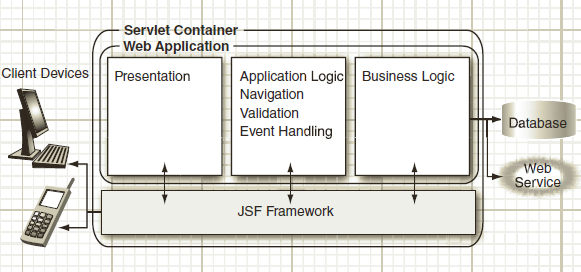
\includegraphics[width=0.5\textwidth]{JSF_architecture.png}
\end{figure}

\end{frame}


\begin{frame}{Comunicazione client-server}

\begin{figure}
	\centering
	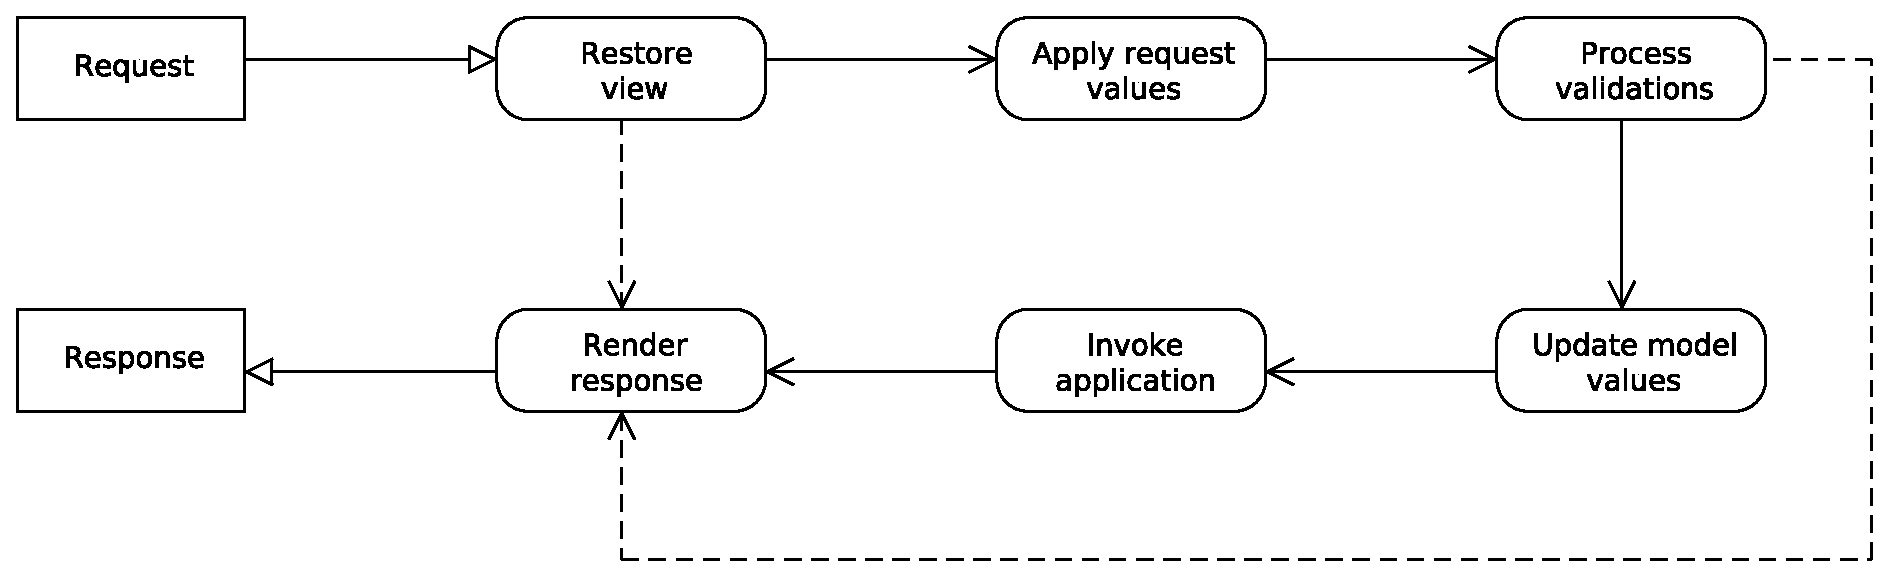
\includegraphics[width=1\textwidth]{custom_JSF_lifecycle.eps}
\end{figure}

\end{frame}


\subsection{Architettura}

\begin{frame}{Architettura tecnologie}
\begin{figure}
	\centering
	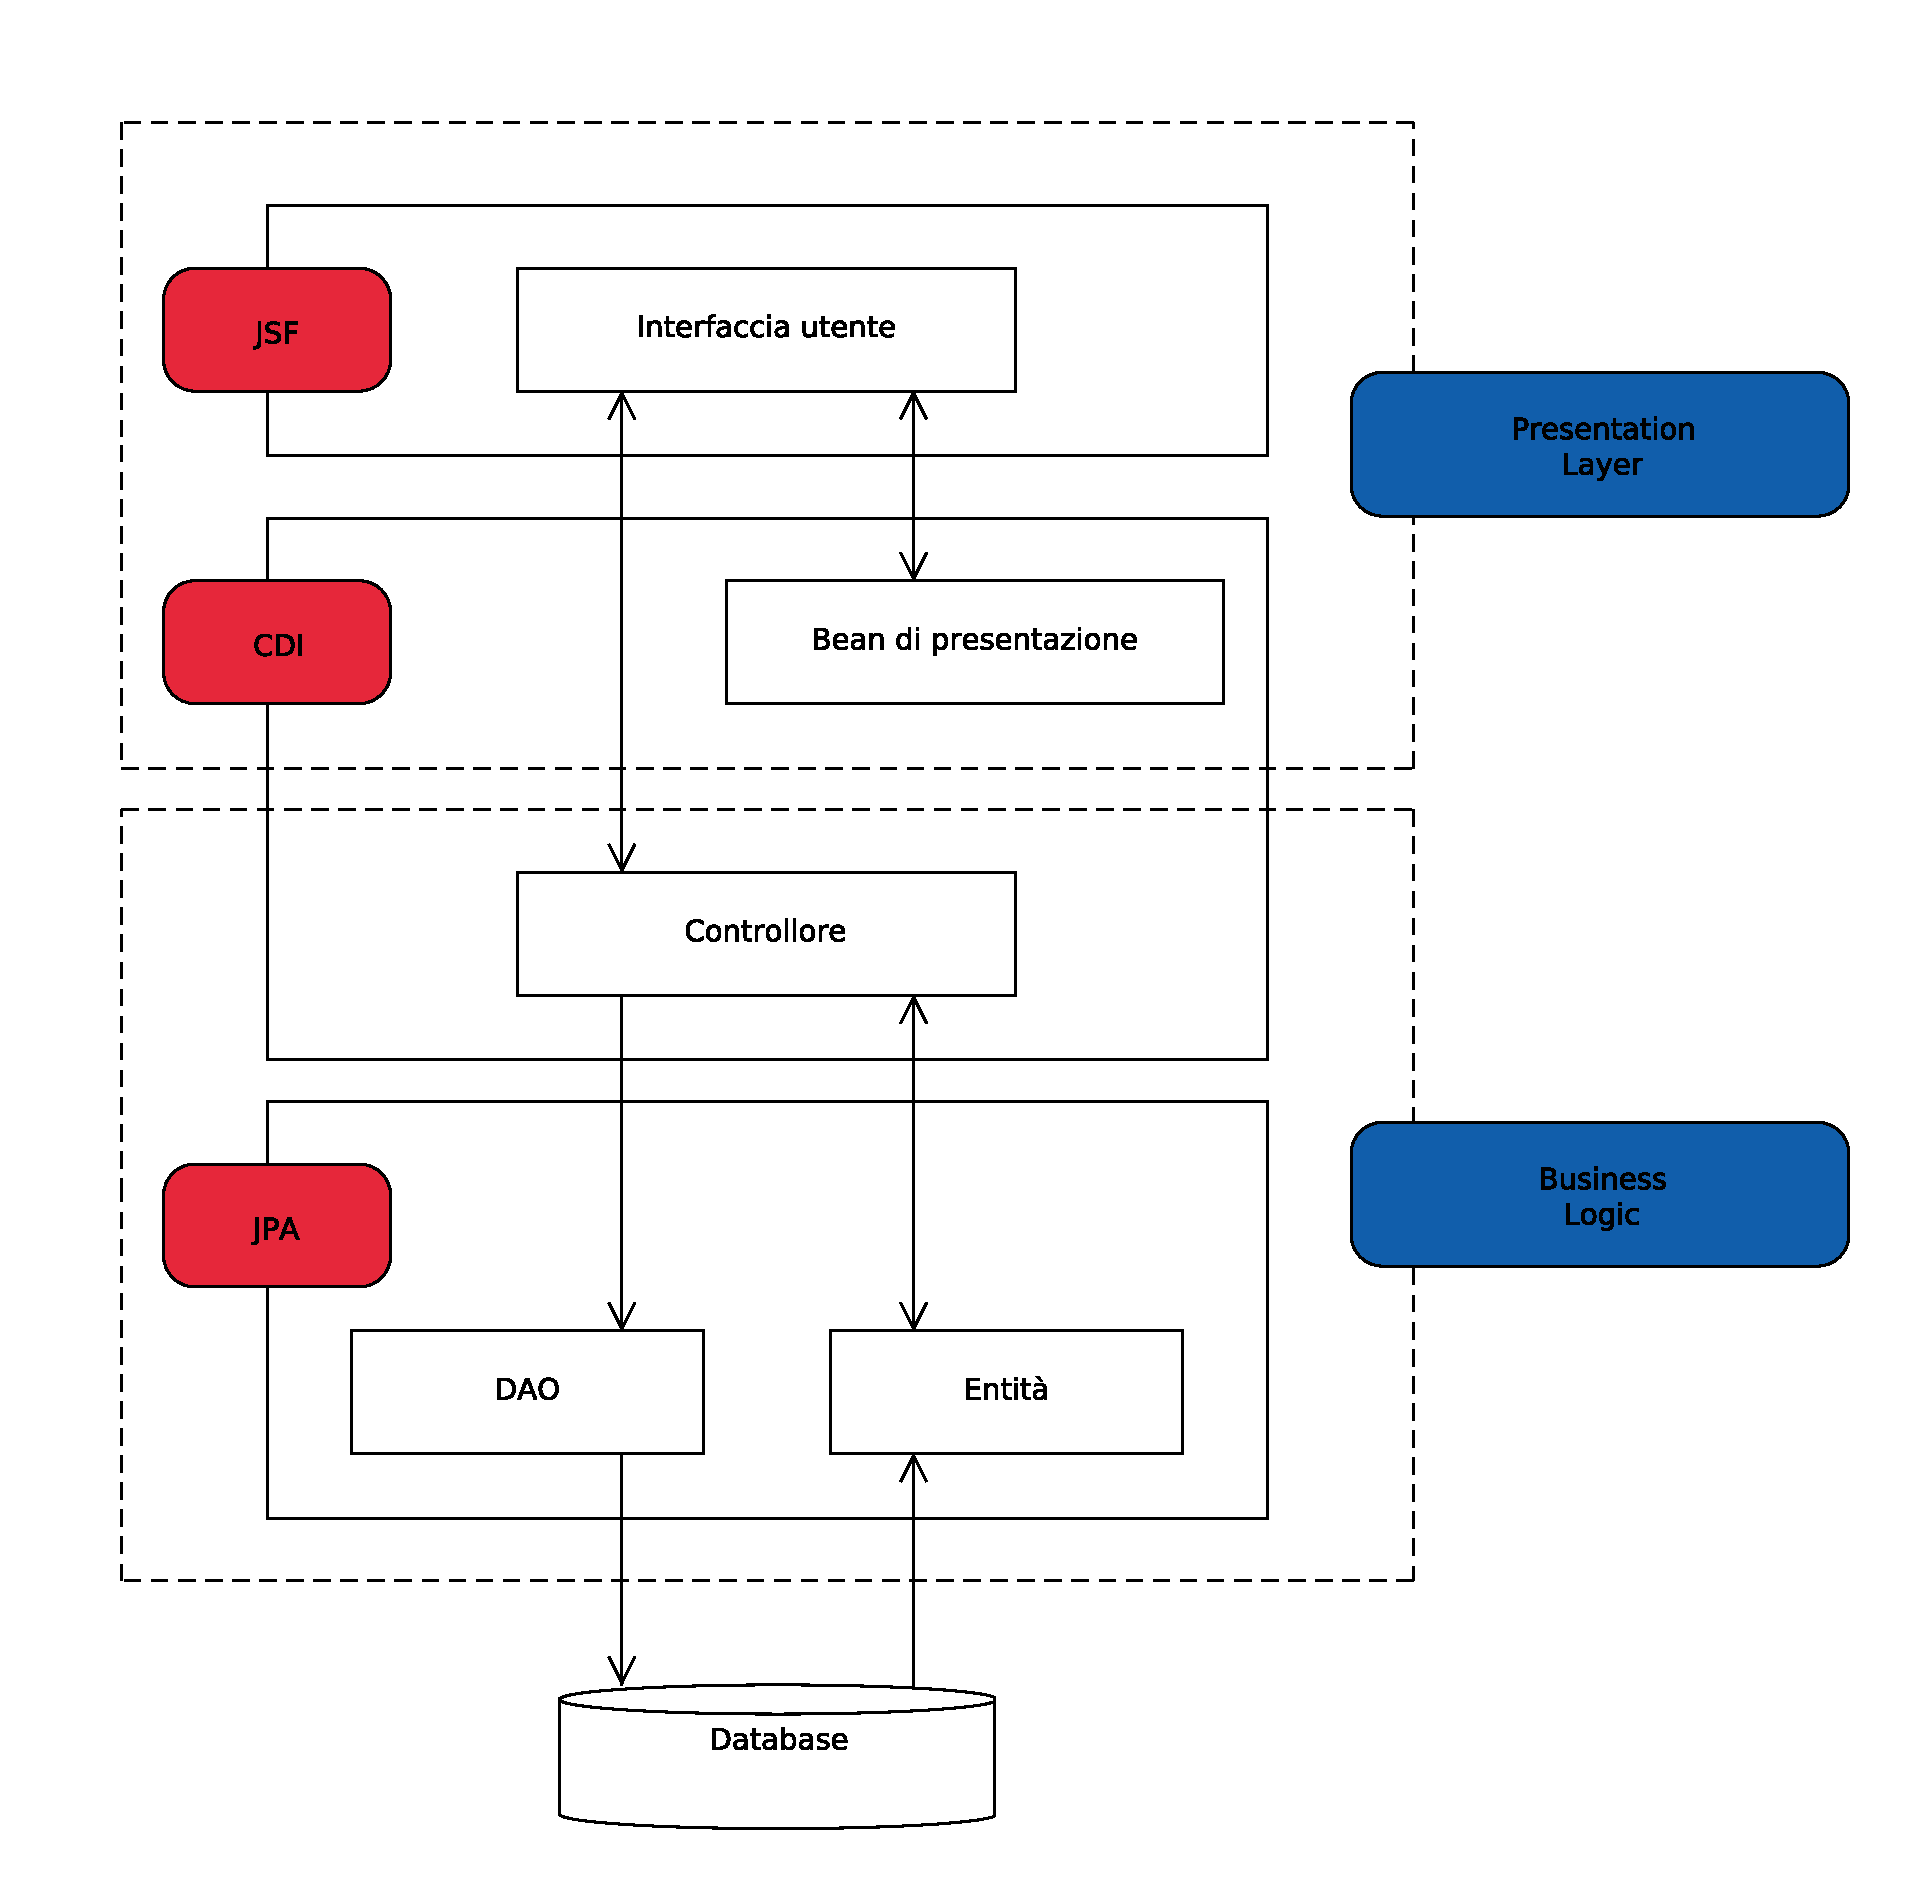
\includegraphics[width=0.6\textwidth]{tech_architecture.eps}
\end{figure}
\end{frame}



